\documentclass[12pt]{article}
\usepackage[english]{babel}
\usepackage{natbib}
\usepackage{url}
\usepackage{hyperref}
\usepackage{minted}
\usepackage{listings}
\usepackage[utf8x]{inputenc}
\usepackage{graphicx}
\graphicspath{{images/}}
\usepackage{fancyhdr}
\usepackage{vmargin}
\setmarginsrb{3 cm}{2.5 cm}{3 cm}{2.5 cm}{1 cm}{1.5 cm}{1 cm}{1.5 cm}
\title{Práctica 1: Mi primer bootloader}% Title 
\author{Meza Madrid Damián}% Author
\date{Enero 2019}% Date
\makeatletter
\let\thetitle\@title
\let\theauthor\@author
\let\thedate\@date
\def\@seccntformat#1{%
  \expandafter\ifx\csname c@#1\endcsname\c@section\else
  \csname the#1\endcsname\quad
  \fi}
\makeatother
\pagestyle{fancy}
\fancyhf{}
\rhead{\theauthor}
\lhead{\thetitle}
\cfoot{\thepage}
\begin{document}

%%%%%%%%%%%%%%%%%%%%%%%%%%%%%%%%%%%%%%%%%%%%%%%%%%%%%%%%%%%%%%%%%%%%%%%%%%%%%%%%%%%%%%%%%

\begin{titlepage}
	\centering
    \vspace*{0.5 cm}
    
\includegraphics[scale = 0.30]{escom.png}\\[1.0 cm]	% University Logo
	\textsc{\Large Instituto Politécnico Nacional}\\[0.5 cm]% Course Code
	\textsc{\Large Escuela Superior de Computo}\\[0.5 cm]% Course Code
	\rule{\linewidth}{0.2 mm} \\[0.4 cm]
	{ \huge \bfseries \thetitle}\\
	\rule{\linewidth}{0.2 mm} \\[1.5 cm]
	Reporte\\
	Profesor: Ulises Velez Saldaña \\
	Alumno: Meza Madrid Raúl Damián\\
    Clase: Sistemas operativos\\
    Grupo: 2CM7\\
\end{titlepage}
\section{Introducción}
A la hora de encender una computadora se ejecuta una secuencia de procesos y eventos, uno de ellos es la ejecución del BIOS que se encarga de revisar el funcionamiento del hardware (que usualmente ya ha sido revisado por la motherboard) para posteriormente buscar el cargador de sistema, bootloader. El bootloader es aquel que,después de ser cargado, busca y carga el sistema operativo; en ocasiones re-escribe parte del BIOS. Para que el bootloader funcione, es necesario que este cumpla ciertos de requisitos.
\begin{itemize}
    \item Debe encontrarse en el primer segmento dentro del disco duro
    \item Debe cargarse en el primer segmento de la memoria RAM 
    \item Debe dejar libres los primero 512 \footnote{El documento p1-minimum-bootloader.pdf especifica un tamaño de 10 bytes mas grandes al especificado por el profesor en clase. Se decidió seguir este ultimo porque tiene mas sentido.} bytes del mismo segmento.
    \item Al final del segmento debe escribir el Magic Number\footnote{El Magic Number es 0xAA55 en hexadecimal y  0b1010101001010101 en binario} para informar al BIOS mostrará un mensaje o leerá el siguiente disco.\cite{MagicNumber}
\end{itemize}
\subsection{Programas y herramientas utilizados}
Esta práctica fue desarrollada en el sistema operativo Ubuntu 18.04.1 LTS. Los programas y herramientas utilizados, junto con el comando de instalación, en caso de que no estuvieran instalados ya. 
\begin{itemize}
    \item NASM : \$ apt-get install nasm
    \item QEMU : \$ apt-get install qemu
    \item dd
\end{itemize}
\section{Objetivo}
Que el alumno aplique la teoría vista en clase, conozca el proceso y las herramientas necesarias para construir el cargados.
\section{Desarrollo}
\subsection{Crear el archivo bootloader.asm}
El archivo bootloader.asm debe cumplir con las siguientes espeficicaciones
\begin{itemize}
    \item Un ciclo infinito.
    \item Compilar en 16 bits.
    \item Rellenar el segmento con ceros hasta una longitud de 510 bytes. 
    \item Colocar el magic number 0xAA55 en la posición 511 y 512.
\end{itemize}
El archivo resultante es el siguiente 
\lstinputlisting[language={[x86masm]Assembler}]{bootloader.asm}
\subsection{Ensamblar}
Ensamblar cargador generando un ejecutable de código máquina plano. Para esto se usara NASM. Los parámetros -f bin especifican el formato de salida como flat binary y se guardan dentro de la carpeta bin con el nombre bootloader. El parámetro resultante es:
\begin{minted}{bash}
nasm src/bootloader.asm  -f bin bin/bootloader
\end{minted}
\subsection{Crear el disco}
Crear el disco con el cargador en el sector cero. En este caso se usara un floppy disk (extinción flp) lleno con ceros (if=/dev/zeros) con 1440 (count=1440) segmentos de tamaño de un megabyte; 1024 bytes (bs=1024).
\begin{minted}{bash}
dd if=/dev/zero of=images/escomos.flp bs=1024 count=1440
\end{minted}
\begin{lstlisting}
 1440+0 records in
 1440+0 records out
 1474560 bytes (1.5 MB, 1.4 MiB) copied,
 0.00708728s, 208 MB/s
\end{lstlisting}
Despues se agrega la información del bootloader que creamos (if = bin/bootloader)
\begin{minted}{bash}
dd if=bin/bootloader of=images/escomos.flp seek=0 count=1 conv=notrunc
\end{minted}
\begin{lstlisting}
 1+0 records in
 1+0 records out
 512 bytes copied, 0.000413659 s, 1.2 MB/s
\end{lstlisting}
\subsection{Correr el sistema}
Correr el sistema operativo en un emulador, en este caso QEMU en un sistema con la arquitectura i386, se especifica el formato -fda como un floppy disk y se carga la imagen creada anteriormente. 
\begin{minted}{bash}
qemu-system-i386 -fda images/escomos.flp 
\end{minted}
El primer resultado es un mensaje en consola que dice:
\begin{lstlisting}
 WARNING: Image format was not specified for 
    'images/escomos.flp'and probing guessed raw.
    Automatically detecting the format is dangerous
    for raw images, write operations  on block 0 
    will be restricted. Specify the 'raw' format
    explicitly to remove the restrictions. 
\end{lstlisting}
y después vemos una pantalla que dice:
\begin{figure}[!htb]
\begin{minipage}{0.5\textwidth}
SeaBIOS (version 1.10.2-1ubuntu1)\\\\
iPXE ( ... )\\
Booting from Hard Disk...\\
Boot failed: could not read the boot disk\\
booting from Floppy\\
\_
\end{minipage}
\begin{minipage}{0.5\textwidth}
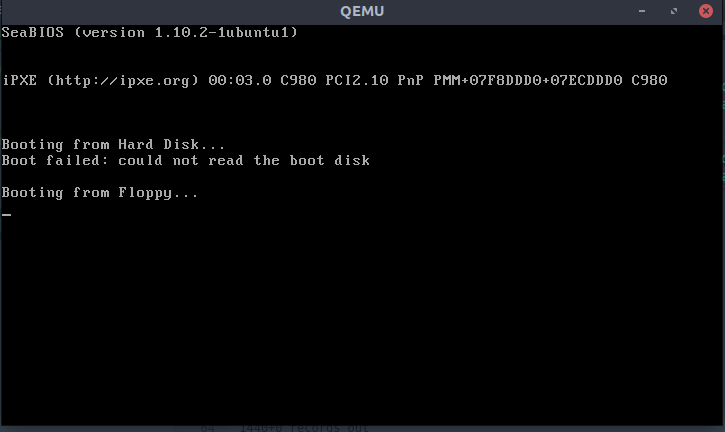
\includegraphics{Prompt.png}
\end{minipage}
\end{figure}
\subsection{Errores y problemas}
La primera vez que se uso el comando NASM, decía que habia mas de una entrada, 
\begin{minted}{bash}
 nasm src/bootloader.asm -f bin bin/bootloader
\end{minted}
\begin{lstlisting}
 nasm: error: more than one input file specified
 type 'nasm -h' for help
\end{lstlisting}
Lo primero que hice fue quitar los argumentos extras, pero recibí el mismo mensaje. Trate de borrar espacios extras, pero tampoco. Termine haciéndolo directo desde la carpeta para después solo copiar el archivo ha la carpeta correspondiente
\begin{minted}{bash}
nasm bootloader.asm -f bin 
\end{minted}
\nocite{*}
\bibliographystyle{plain}
\bibliography{biblist}
\end{document}

